%md->tex->template
\documentclass[12pt]{article}
\usepackage{CJKutf8}
\usepackage{amsmath}
\usepackage{geometry}
\usepackage{fancyhdr}
\usepackage{longtable,booktabs}
\usepackage{enumerate}
\usepackage{enumitem}
\usepackage{amsthm}
\usepackage{amssymb}
\usepackage{tikz}
\setlist[enumerate,1]{font=\bfseries}
\geometry{left=3.0cm,right=2.0cm,top=3.0cm,bottom=3.0cm}

\newenvironment{firstlayer}%
{\begin{list}{}{\renewcommand{\makelabel}[1]{\textbf{##1}.\hfil}
}}
{\end{list}}
\newenvironment{secondlayer}%
{\begin{list}{}{\renewcommand{\makelabel}[1]{(##1)\hfil}
}}
{\end{list}}

\renewcommand{\proofname}{\textbf{证明}}

\providecommand{\sol}{\textbf{解}.~}

\title{第 10 次作业}
\author{Log Creative}
\date{May 16, 2020}
\begin{document}

\begin{CJK}{UTF8}{gbsn}

\maketitle

\begin{firstlayer}
  \item[4]设$A=\{1,2,3\}$,在$A$上有多少种不同的关系?设$\mid A\mid=n$,在$A$上有多少种不同的关系?

\sol 3个元素之间的关系可以组成$3^2=9$对,每一对都可以有相连(1)和不相连(0),所以共有$2^9=512$种关系。

如果$\mid A\mid=n$,则有$2^{n^2}$种关系。

\item[7]对$A=\{0,1,2,3,4\}$上的下列关系,给出关系图和关系矩阵。
\begin{secondlayer}
  \item[2]$R_2=\{ \langle x,y \rangle \mid 0\leq x-y<3 \}$

\sol
$\left(\begin{matrix}
    1 & 0 & 0 & 0 & 0 \\
    1 & 1 & 0 & 0 & 0 \\
    1 & 1 & 1 & 0 & 0 \\
    0 & 1 & 1 & 1 & 0 \\
    0 & 0 & 1 & 1 & 1 \\
\end{matrix}\right)$

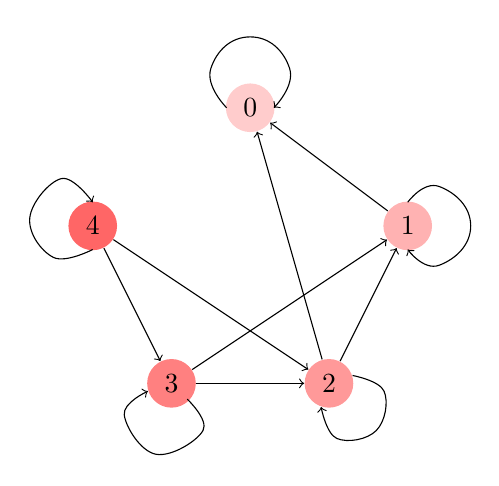
\begin{tikzpicture}

\node[circle, fill=red!20] (v1) at (-0.5,2.5) {0}  ;
\node[circle, fill=red!30] (v2) at (1.5,1) {1};
\node[circle, fill=red!40] (v3) at (0.5,-1) {2};
\node[circle, fill=red!50] (v4) at (-1.5,-1) {3};
\node[circle, fill=red!60] (v5) at (-2.5,1) {4};
\node (v1a) at (-0.5,3.4) {};

\draw[->]  (v2) edge (v1);
\draw[->]   (v3) edge (v2);
\draw[->]  (v4) edge (v3);
\draw[->]  (v5) edge (v4);
\draw[->]  (v3) edge (v1);
\draw[->]  (v4) edge (v2);
\draw[->]  (v5) edge (v3);
%还差5个自环


\draw[->]  plot[smooth, tension=.9] coordinates {(-0.8,2.5) (-1,3) (v1a) (0,3) (-0.2,2.5)};
\draw[->]  plot[smooth, tension=.9] coordinates {(1.5,1.3) (1.9,1.5) (2.3,1) (1.9,0.5) (1.5,0.7)};
\draw[->]  plot[smooth, tension=.7] coordinates {(0.8,-0.9) (1.2,-1.1) (1.1,-1.6) (0.6,-1.7) (0.4,-1.3)};
\draw[->]  plot[smooth, tension=.7] coordinates {(-1.3,-1.2) (-1.1,-1.6) (-1.7,-1.9) (-2.1,-1.4) (-1.8,-1.1)};
\draw[->]  plot[smooth, tension=.7] coordinates {(-2.5,0.7) (-3,0.6) (-3.3,1.1) (-2.9,1.6) (-2.5,1.3)};
\end{tikzpicture}

\end{secondlayer}
\item[9] 设$A=\{\langle \varnothing,\{ \varnothing,\{ \varnothing \} \} \rangle ,\langle \{ \varnothing \},\varnothing \rangle  \}$,写出$A\circ A,A^{-1},A\uparrow \varnothing,A\uparrow\{\varnothing\},A\uparrow\{\varnothing,\{ \varnothing \}\},A[\varnothing]$ $,A[\{ \varnothing \}],A[\{\varnothing, \{ \varnothing\}\}]$。

\sol 
\begin{align*}
  A\circ A&=\{ \langle \{ \varnothing \}, \{ \varnothing,\{ \varnothing \} \}\rangle \}\\
A^{-1}&=\{\langle \{ \varnothing,\{ \varnothing \} \},\varnothing \rangle ,\langle \varnothing,\{ \varnothing \} \rangle  \}\\
A\uparrow \varnothing&=\varnothing &&\text{因为$\varnothing$中没有元素。}\\
A\uparrow\{\varnothing\}&=\{\langle \varnothing,\{ \varnothing,\{ \varnothing \} \} \rangle\}\\
A\uparrow\{\varnothing,\{ \varnothing \}\}&=\{\langle \varnothing,\{ \varnothing,\{ \varnothing \} \} \rangle ,\langle \{ \varnothing \},\varnothing \rangle  \}=A\\
A[\varnothing]&=\varnothing &&\text{因为$\varnothing$中没有元素。}\\
A[\{ \varnothing \}]&=\{\{ \varnothing,\{ \varnothing \} \}\}\\
A[\{\varnothing, \{ \varnothing\}\}]&=\{\{ \varnothing,\{ \varnothing \} \},\varnothing \}
\end{align*}

\item[13] 对$A$到$B$的关系$R$,$a\in A$,定义$B$的一个子集$R(a)=\{b\mid aRb\}$。

在 $C=\{-4,-3,-2,-1,0,1,2,3,4\}$ 上定义

\begin{align*}
R&=\{ \langle x,y \rangle \mid x<y\}\\S&=\{ \langle x,y \rangle\mid x-1<y<x+2 \}\\T&=\{ \langle x,y \rangle \mid x^2\leq y \}
\end{align*}

写出集合$R(0),R(1),S(0),S(-1),T(0),T(-1)$。

\sol \begin{align*}
       R(0)&=\{1,2,3,4\}\\R(1)&=\{2,3,4\}\\S(0)&=\{0,1 \}\\S(-1)&=\{ -1,0 \}\\T(0)&=\{0,1,2,3,4\}\\T(-1)&=\{1,2,3,4\}
     \end{align*}


\end{firstlayer}

\end{CJK}

\end{document}

